
\chapter{Distributed Non-Linear Measurement Fusion with Untrusted Participants}\label{ch:nonlin_fusion}

% 
% 8888888b.  8888888b.   .d88888b.  888888b.   
% 888   Y88b 888   Y88b d88P" "Y88b 888  "88b  
% 888    888 888    888 888     888 888  .88P  
% 888   d88P 888   d88P 888     888 8888888K.  
% 8888888P"  8888888P"  888     888 888  "Y88b 
% 888        888 T88b   888     888 888    888 
% 888        888  T88b  Y88b. .d88P 888   d88P 
% 888        888   T88b  "Y88888P"  8888888P"  
%                                              
%                                              
%                                              
% 

\section{Problem Formulation}\label{sec:nonlin_fusion:problem}
This problem aims to lay down a foundation for solving general non-linear measurement fusion where sensor and navigator privacy is preserved and involved data remains confidential. Since solving the general problem is difficult due to broad measurement definitions and the need for concrete communications to be known when proving cryptographic aims, we study a specific non-linear problem instead. The presented solution to this problem then lends itself to solving a class of related, but not exhaustive, non-linear measurement fusion problems with the same communication and cryptographic requirements, discussed later in this chapter. We consider the specific context of confidential range sensor navigation, where no sensor is to learn any information about the navigator or other sensors beyond their local measurements, while the navigator learns no information about individual sensors beyond its location estimate. The problem is two-fold, in that we require explicit cryptographic requirements with a suitable encryption scheme meeting them as well as an estimation scheme that can use the encryption in the context of range-only navigation.

To give a formal cryptographic requirement in a distributed setting, we first consider the communication requirements of our context and define attacker capabilities and the desired security of a suitable encryption scheme. In this section, we define a communication protocol and the relevant formal definition of security we aim to achieve, followed by the estimation problem to which we will apply it.

% 
%  ######  ########  ##    ## ########  ########  #######     ########  ########   #######  ########  
% ##    ## ##     ##  ##  ##  ##     ##    ##    ##     ##    ##     ## ##     ## ##     ## ##     ## 
% ##       ##     ##   ####   ##     ##    ##    ##     ##    ##     ## ##     ## ##     ## ##     ## 
% ##       ########     ##    ########     ##    ##     ##    ########  ########  ##     ## ########  
% ##       ##   ##      ##    ##           ##    ##     ##    ##        ##   ##   ##     ## ##     ## 
% ##    ## ##    ##     ##    ##           ##    ##     ##    ##        ##    ##  ##     ## ##     ## 
%  ######  ##     ##    ##    ##           ##     #######     ##        ##     ##  #######  ########  
% 

\subsection{Formal Cryptographic Problem}\label{subsec:nonlin_fusion:crypto_problem}
The communication between the navigator and sensors in our estimation problem will be decomposed into a simple two-step bi-directional protocol that will simplify defining formal security. In section \ref{subsec:nonlin_fusion:localisation}, we will show how this protocol is sufficient to compute the location estimate at a navigator while meeting our desired privacy goals. The communication protocol is as follows.

At every \textit{instance} $t$ (used to distinguish from an estimation \textit{timestep}), the navigator first broadcasts $l$ weights $\theta_j^{(t)}$, $1\leq j\leq l$ to all sensors $i$, $1\leq i \leq n$, who individually compute linear combinations $e^{(t)}_i=\sum^l_{j=1}a_{j,i}^{(t)}\theta_i^{(t)}$ based on their measurement data $a_{j,i}$. Linear combinations are then sent back to the navigator, who computes their sum $\sum^n_{i=1}e^{(t)}_{i}$. This two-step linear combination aggregation protocol has been visually displayed in figure \ref{fig:nonlin_fusion:aggregation_steps}.
\begin{figure}[htbp]
\centering
\begin{tikzpicture}[font=\footnotesize,scale=0.95]
    % Step 1
    \node at (3.25,5.5) {1. Broadcast and Combination Step};
    % Navigator
    \fill (3.25,4.75) [pyplotblue!70] ellipse (0.4 and 0.4);
    \pic[xscale=0.22,yscale=0.3] at (3.25,4.9225) {plane};
    % Sensors
    \node at (1.5,1.375) {Sensor $1$};
    \fill [pyplotorange!70] (0.25,1.625) rectangle (2.875,2.625);
    \node at (1.625,2.125) {$\displaystyle l_1^{(t)} \!=\! \sum^m_{j=1}a_{1,j}^{(t)}\omega_j^{(t)}$};
    \node at (5,1.375) {Sensor $n$};
    \fill [pyplotorange!70] (3.625,1.625) rectangle (6.25,2.625);
    \node at (5,2.125) {$\displaystyle l_n^{(t)} \!=\! \sum^m_{j=1}a_{n,j}^{(t)}\omega_j^{(t)}$};
    \fill [black] (3.5,2.125) circle (0.05);
    \fill [black] (3,2.125) circle (0.05);
    \fill [black] (3.25,2.125) circle (0.05);
    % Lines
    \draw [-latex] plot[smooth, tension=.7] coordinates {(3.5,4.25) (5,2.875)};
    \draw [-latex] plot[smooth, tension=.7] coordinates {(3,4.25) (1.5,2.875)};
    \fill [lightgray] (2.125,3.875) rectangle (4.375,3.125);
    \node at (3.25,3.5) {$\langle\omega_1^{(t)},\dots ,\omega_m^{(t)}\rangle$};
    
    % Step 2
    \node at (3.25,0.25) {2. Aggregation Step};
    % Navigator
    \fill [pyplotblue!70] (1.375,-2) rectangle (5.125,-0.25);
    \pic[xscale=0.22,yscale=0.3] at (3.25,-0.4775) {plane};
    \node at (3.25,-1.375) {$\displaystyle \sum^{n}_{i=1}\sum^{m}_{j=1} a_{i,j}^{(t)}\omega_j^{(t)} = \sum^n_{i=1}l^{(t)}_{i}$};
    % Sensors
    \node at (1.25,-3.875) {Sensor $1$};
    \fill  (5.25,-3.25) [pyplotorange!70] ellipse (0.4 and 0.4);
    \node at (5.25,-3.875) {Sensor $n$};
    \fill  (1.25,-3.25) [pyplotorange!70] ellipse (0.4 and 0.4);
    \fill [black] (2.75,-3.25) circle (0.05);
    \fill [black] (3.75,-3.25) circle (0.05);
    \fill [black] (3.25,-3.25) circle (0.05);
    % Lines
    \draw [-latex] plot[smooth, tension=.7] coordinates {(5,-2.75) (4.5,-2.25)};
    \draw [-latex] plot[smooth, tension=.7] coordinates {(1.5,-2.75) (2,-2.25)};
    \fill [lightgray] (1.625,-2.5) rectangle (2.25,-3);
    \node at (2,-2.75) {$l_1^{(t)}$};
    \fill [lightgray] (4.25,-2.5) rectangle (4.875,-3);
    \node at (4.625,-2.75) {$l_n^{(t)}$};
    
    % Bounding rectangles
    \draw [gray] (0,6) rectangle (6.5,1);
    \draw [gray] (0,0.75) rectangle (6.5,-4.25);
\end{tikzpicture}
\caption{Required linear combination aggregation steps at instance $t$.}
\label{fig:nonlin_fusion:aggregation_steps}
% TODO make two subfigures instead. Current text labels should be figure captions. No bounding boxes required. Update variables as well
\end{figure}
In addition, we note that an alternative approach to the two-step protocol is computing $\sum^{l}_{j=1}(\theta_j^{(t)}\sum^{n}_{i=1} a_{i,j}^{(t)})$ at the navigator, requiring only values $a_{i,j}^{(t)}$, $1\leq j \leq l$ to be sent from each sensor $i$. We justify the use of bi-directional communication by reducing communication costs when the number of weights is larger than the number of sensors, $l>n$, and by sending fewer weights in the presence of repeats, as will be shown to be the case in section \ref{subsec:nonlin_fusion:localisation}.

Before giving a formal definition for the construction and security of our desired encryption scheme, we make the following assumptions about the capabilities of the participants.
\begin{description}
    \item[Global Navigator Broadcast] We assume that broadcast information from the navigator is received by \textit{all} sensors involved in the protocol.
    \item[Consistent Navigator Broadcast] We assume that broadcast information from the navigator is received equally by all sensors. This means the navigator may not send different weights to individual sensors during a single instance $t$.
    \item[Honest-but-Curious Sensors] We adopt the honest-but-curious attacker model for all involved sensors, meaning that they follow the localisation procedure correctly but may store or use any gained sensitive information.
\end{description}
We justify the global broadcast assumption by noting that any subset of sensors within the range of the navigator can be considered a group and treated as the global set during estimation, generalising the method, while the widespread use of cheap non-directional antennas supports the assumption of consistent broadcasts. The final assumption refers to the known problem of misbehaving sensors [lazosSeRLocSecureRangeindependent2004,ben-galOutlierDetection2005], often requiring additional complicated detection mechanisms, and will not be considered in this chapter.

We are now ready to define the type of encryption scheme we want for the specified communication protocol and the security guarantees it should provide. We let a linear combination aggregation scheme be defined as a tuple of the four algorithms $(\mathsf{Setup}, \mathsf{Enc}, \mathsf{CombEnc}, \mathsf{AggDec})$. These will be used by a trusted setup party, the navigator, and sensors $1\leq i\leq n$. They are defined as follows.
\begin{description}
    \item[$\mathsf{Setup}(\kappa)$] On input of security parameter $\kappa$, generate public parameters $\mathsf{pub}$, the number of weights $l$, the navigator's public and private keys $\mathsf{pk}_{\mathsf{a}}$ and $\mathsf{sk}_{\mathsf{a},0}$ and the sensor private keys $\mathsf{sk}_{\mathsf{a},i}$, $1\leq i\leq n$.
    \item[$\mathsf{Enc}(\mathsf{pk}_{\mathsf{a}}, x)$] The navigator and sensors can encrypt any value $x\in\mathbb{Z}$ with the navigator's public key $\mathsf{pk}_{\mathsf{a}}$ and obtain the encryption $\mathcal{E}_{\mathsf{pk}_{\mathsf{a}}}(x)$.
    \item[$\mathsf{CombEnc}(t, \mathsf{pk}_{\mathsf{a}}, \mathsf{sk}_{\mathsf{a},i}, \mathcal{E}_{\mathsf{pk}_{\mathsf{a}}}(\theta_1^{(t)}),\dots,\mathcal{E}_{\mathsf{pk}_{\mathsf{a}}}(\theta_l^{(t)}), a^{(t)}_{i,1},\dots,a^{(t)}_{i,l})$] At instance $t$, sensor $i$ computes and obtains the encrypted linear combination denoted $e^{(t)}_i = \mathcal{E}_{\mathsf{pk}_{\mathsf{a}},\mathsf{sk}_{\mathsf{a},i}}(\sum^l_{j=1}a^{(t)}_{i,j}\theta^{(t)}_j)$ using its secret key $\mathsf{sk}_{\mathsf{a},i}$.
    \item[$\mathsf{AggDec}(t, \mathsf{pk}_{\mathsf{a}}, \mathsf{sk}_{\mathsf{a},0}, e^{(t)}_1,\dots,e^{(t)}_n)$] At instance $t$, the navigator computes the aggregation of linear combinations $\sum^{n}_{i=1}e_i^{(t)}=\sum^{n}_{i=1}\sum^{l}_{j=1} a^{(t)}_{i,j}\theta^{(t)}_j$ using its public and private keys $\mathsf{pk}_{\mathsf{a}}$, $\mathsf{sk}_{\mathsf{a},0}$.
\end{description}
The security notions we want these algorithms to meet reflect the previously stated estimation privacy goals. The navigator should learn no information from individual sensors while sensors should learn no information from the navigator or any other sensors. In the context of the introduced communication protocol, this can be summarised as the following notions.
\begin{description}
    \item[Indistinguishable Weights] No colluding subset of sensors gains any new knowledge about the navigator weights $\theta^{(t)}_j$, $1\leq j\leq l$ when receiving only their encryptions from the current and previous instances and having the ability to encrypt plaintexts of their choice.
    \item[Linear Combination Aggregator Obliviousness] No colluding subset \textit{excluding} the navigator gains additional information about the remaining sensor values to be weighted, $a^{(t)}_{i,j}$, $1\leq j\leq l$, where sensor $i$ is not colluding, given only encryptions of their linear combinations $e_i$ from the current and previous instances. Any colluding subset \textit{including} the navigator learns only the sum of all linear combinations weighted by weights of their choice, $\sum^{n}_{i=1}e_i^{(t)}=\sum^{n}_{i=1}\sum^{l}_{j=1} a^{(t)}_{i,j}\theta^{(t)}_j$.
\end{description}
While indistinguishable weights can be achieved by encrypting weights with an encryption scheme meeting the IND-CPA notion introduced in section \ref{subsec:prelims:crypto_notions}, the novel notion of Linear Combination Aggregator Obliviousness (LCAO) has been formalised as a typical cryptographic game between attacker and challenger in the appendix [app:lcao]. Lastly, we conclude the cryptographic problem definition with the following important remark.
\begin{remark}
    A leakage function including weights from the navigator requires extra care to be taken when giving its definition. If an attacker compromises the navigator, they have control over the weights, and therefore the leakage function. We note that in the leakage function above, $\sum^n_{i=1}\sum^l_{j=1}a^{(t)}_{i,j}\theta^{(t)}_j$, an individual sum weighted by the same weight may be learnt by an attacker, \textit{e.g.}, $\sum^n_{i=1}a^{(t)}_{i,1}$ given weights $(1,0,\dots,0)$, but that individual sensor values $a^{(t)}_{i,j}$ remain private due to the assumption of a consistent broadcast.
\end{remark}

% 
% ########  ######  ########    ########  ########   #######  ########  
% ##       ##    ##    ##       ##     ## ##     ## ##     ## ##     ## 
% ##       ##          ##       ##     ## ##     ## ##     ## ##     ## 
% ######    ######     ##       ########  ########  ##     ## ########  
% ##             ##    ##       ##        ##   ##   ##     ## ##     ## 
% ##       ##    ##    ##       ##        ##    ##  ##     ## ##     ## 
% ########  ######     ##       ##        ##     ##  #######  ########  
% 

\subsection{Estimation problem}\label{subsec:nonlin_fusion:estimation_problem}
The estimation problem we consider, for which we will reformulate communication to the protocol above, is localisation with range-only sensors. In this work, we will focus on the two-dimensional case for simplicity but will derive methods suitable for extension to a three-dimensional equivalent. The state that we wish to estimate must capture the navigator position, $x$ and $y$, and may contain any other components relevant to the system. It is of the form
\begin{equation}
    \vec{x} = 
    \begin{bmatrix}
        x & y & \cdots
    \end{bmatrix}^\top\,. \label{eqn:state_definition}
\end{equation}
This state evolves following some known system model, which at timestep $k$ can be written as
\begin{equation}
    \vec{x}_k = \vec{f}_k(\vec{x}_{k-1}, \vec{w}_k)\,, \label{eqn:system_model}
\end{equation}
with noise term $\vec{w}_k$. Measurements of $\vec{x}_k$ follow a measurement model dependent on sensor $i\in\{1,\dots,n\}$, given by 
\begin{equation}
    z_{k,i} = h_i(\vec{x}_k)+v_{k,i}\,, \label{eqn:measurement_model}
\end{equation}
with Gaussian measurement noises $v_{k,i} \sim \mathcal{N}(0,r_{k,i})$ and measurement function
\begin{equation}
    \begin{split}
        h_i(\vec{x}) &= \left\lVert
        \begin{bmatrix}
            x & y
        \end{bmatrix}^\top
        - \vec{s}_{i}\right\rVert \\
        &= \sqrt{(x-s_{x,i})^2 + (y-s_{y,i})^2}\,,
    \end{split}
\end{equation}
where
\begin{equation}
    \vec{s}_i = 
    \begin{bmatrix}
        s_{x,i} & s_{y,i}
    \end{bmatrix}^\top
\end{equation} 
is the location of sensor $i$.

We aim to provide a filter that estimates the navigator's state $\vec{x}_k$, at every timestep $k$, without learning sensor positions $\vec{s}_i$, measurements $z_{k,i}$ and measurement variances $r_{k,i}$ beyond the information in the corresponding aggregation leakage function. Similarly, sensors should not learn any information about current state estimates or any other sensor information. Leakage will be further discussed in section \ref{subsec:leakage}, but we note that from any sequential state estimates, following known models, some sensor information leakage can be computed by the navigator. In the context of our leakage function, we will show that this corresponds to the global sums of private sensor information, while individual, or subsets of sensors', information remains private. Similarly, corrupted sensors with access to one or more measurements can produce state estimates of their own, leaking information about navigator state estimates, however, the most accurate estimates, requiring all measurements, will always remain private to the navigator.

% 
% 8888888b.         d8888 888b    888  .d8888b.  8888888888      888      .d88888b.   .d8888b.  
% 888   Y88b       d88888 8888b   888 d88P  Y88b 888             888     d88P" "Y88b d88P  Y88b 
% 888    888      d88P888 88888b  888 888    888 888             888     888     888 888    888 
% 888   d88P     d88P 888 888Y88b 888 888        8888888         888     888     888 888        
% 8888888P"     d88P  888 888 Y88b888 888  88888 888             888     888     888 888        
% 888 T88b     d88P   888 888  Y88888 888    888 888             888     888     888 888    888 
% 888  T88b   d8888888888 888   Y8888 Y88b  d88P 888             888     Y88b. .d88P Y88b  d88P 
% 888   T88b d88P     888 888    Y888  "Y8888P88 8888888888      88888888 "Y88888P"   "Y8888P"  
%                                                                                               
%                                                                                               
%                                                                                               
% 

\section{Confidential Range-Only Localisation}\label{subsec:nonlin_fusion:conf_range_only_localisation}

% 
% ##        ######     ###        ######   ######  ##     ## ######## ##     ## ######## 
% ##       ##    ##   ## ##      ##    ## ##    ## ##     ## ##       ###   ### ##       
% ##       ##        ##   ##     ##       ##       ##     ## ##       #### #### ##       
% ##       ##       ##     ##     ######  ##       ######### ######   ## ### ## ######   
% ##       ##       #########          ## ##       ##     ## ##       ##     ## ##       
% ##       ##    ## ##     ##    ##    ## ##    ## ##     ## ##       ##     ## ##       
% ########  ######  ##     ##     ######   ######  ##     ## ######## ##     ## ######## 
% 

\subsection{A Linear Combination Aggregation Scheme}\label{subsec:nonlin_fusion:lcao_scheme}
In this section, we introduce an encryption scheme meeting the desired security properties in section \ref{subsec:crypto_problem}. The scheme is a combination of the Paillier and Joye-Libert schemes and provides encrypted weights meeting IND-CPA and encrypted aggregation meeting the notion of LCAO defined in section~\ref{subsec:crypto_problem}. Similarly to its constituents, the scheme bases its security on the DCRA and, as with the Joye-Libert scheme, requires a trusted party for initial key generation and distribution. 

As aggregation is typically performed on scalar inputs, we extend our notation to the context of multidimensional estimation data by letting an instance $t_{k,\tau}$ uniquely capture the scalar aggregation during an estimation timestep $k$ for a single element with position index $\tau$. To achieve this in practice, any injective function can be used, such as the concatenation $t_{k,\tau}=k\mathbin\|\tau$. The four algorithms defining our scheme are given as follows.
\begin{description}
    \item[$\mathsf{Setup}(\kappa)$] On input parameter $\kappa$, generate two equal-length, sufficiently large, primes $p$ and $q$, and compute $N=pq$. Define a hash function $H:\mathbb{Z} \rightarrow \mathbb{Z}_{N^2}^*$, choose the number of weights to combine, $m>1$, and set public parameter $\mathsf{pub}=H$, navigator public key $pk_0 = N$ and navigator private key $sk_0=(p,q)$. Sensor secret keys are generated by choosing $sk_i,\,i\in\{1,\dots,n-1\}$ uniformly from $\mathbb{Z}_{N^2}$ and setting the last key to $sk_n = -\sum^{n-1}_{i=1}sk_i$.
 
    \item[$\mathsf{Enc}(pk_0, x)$] Public-key encryption is computed by the Paillier encryption scheme with implicit generator $g=N+1$. This is given by
    \begin{equation}
        \mathcal{E}_{pk_0}(x) = (N+1)^{x}\rho^N \pmod{N^2}\,, \label{eqn:our_scheme_encrypt}
    \end{equation}
    for a randomly chosen $\rho \in \mathbb{Z}_N$.

    \item[$\mathsf{CombEnc}(t_{k,\tau}, pk_0, sk_i, \mathcal{E}_{pk_0}(\omega_1^{(k,\tau)})\dots , a^{(k,\tau)}_{i,1}\dots )$] At the instance $t_{k,\tau}$, encrypted linear combination is given by 
    \begin{equation}
        l^{(k,\tau)}_i = H(t_{k,\tau})^{sk_i}\prod^{m}_{j=1}\mathcal{E}_{pk_0}(\omega^{(k,\tau)}_j)^{a^{(k,\tau)}_{i,j}} \pmod{N^2}\,,\label{eqn:our_scheme_lin_comb}
    \end{equation}
    and makes use of the homomorphic property \eqref{eqn:paillier_hom_mult}. Correctness follows from
    \begin{equation*}
        \begin{split}
            l^{(k,\tau)}_i &= H(t_{k,\tau})^{sk_i}\prod^{m}_{j=1}\mathcal{E}_{pk_0}(\omega^{(k,\tau)}_j)^{a^{(k,\tau)}_{i,j}} \pmod{N^2} \\
            &= H(t_{k,\tau})^{sk_i}\prod^{m}_{j=1}\mathcal{E}_{pk_0}(a^{(k,\tau)}_{i,j}\omega^{(k,\tau)}_j) \pmod{N^2} \\
            &= H(t_{k,\tau})^{sk_i}\cdot \\
            &\qquad \prod^{m}_{j=1}(N+1)^{a^{(k,\tau)}_{i,j}\omega^{(k,\tau)}_j} \rho^{N}_{j} \pmod{N^2} \\
            &= H(t_{k,\tau})^{sk_i}\cdot \\
            &\qquad (N+1)^{\sum^{m}_{j=1}a^{(k,\tau)}_{i,j}\omega^{(k,\tau)}_j} \tilde{\rho}_{i}^{N} \pmod{N^2}\,,
        \end{split}
    \end{equation*}
    for some values $\rho_j \in \mathbb{Z}_N,\,j\in\{1,\dots,m\}$ and $\tilde{\rho}_i=\prod^{m}_{j=1}\rho_j$. Here, $\tilde{\rho}_i^N$ and $H(t_{k,\tau})^{sk_i}$ can be considered the noise terms corresponding to the two levels of encryption from $pk_0$ and $sk_i$, respectively.

    \item[$\mathsf{AggDec}(t_{k,\tau}, pk_0, sk_0, l^{(k,\tau)}_1,\dots,l^{(k,\tau)}_n)$] Aggregation is computed as $l^{(k,\tau)} = \prod^n_{i=1}l^{(k,\tau)}_i \pmod{N^2}$, removing the aggregation noise terms, and is followed by Paillier scheme decryption
    \begin{equation}
        \begin{split}
            \sum^{n}_{i=1}\sum^{m}_{j=1}&a^{(k,\tau)}_{i,j}\omega^{(k,\tau)}_j =\\
            &\frac{L((l^{(k,\tau)})^\lambda\pmod{N^2})}{L((N+1)^\lambda\pmod{N^2})} \pmod{N}\,,
        \end{split} \label{eqn:our_scheme_decrypt}
    \end{equation}
    with $\lambda = \mathsf{lcm}(p-1, q-1)$ and $L(\psi) = \frac{\psi-1}{N}$. The correctness of the aggregation can be seen from
    \begin{align*}
        \begin{split}
        l^{(k,\tau)} &= \prod^n_{i=1}H(t_{k,\tau})^{sk_i}\cdot \\
        &\qquad (N+1)^{\sum^{m}_{j=1}a^{(k,\tau)}_{i,j}\omega^{(k,\tau)}_j}\tilde{\rho}_i^N \!\!\pmod{N^2}
        \end{split}\\
        \begin{split}
            &= H(t_{k,\tau})^{\sum^n_{i=1}sk_i}\cdot \\
            &\qquad \prod^n_{i=1}(N+1)^{\sum^{m}_{j=1}a^{(k,\tau)}_{i,j}\omega^{(k,\tau)}_j}\tilde{\rho}_i^N \!\!\pmod{N^2}
        \end{split}\\
        &= (N+1)^{\sum^n_{i=1}\sum^{m}_{j=1}a^{(k,\tau)}_{i,j}\omega^{(k,\tau)}_j}\tilde{\rho}^N \!\!\pmod{N^2}\,,
    \end{align*}
    for some values $\tilde{\rho}_i \in \mathbb{Z}_N,\,i\in\{1,\dots,n\}$ and $\tilde{\rho}=\prod^{n}_{i=1}\tilde{\rho}_i$.
\end{description}
Additionally, we note that in the above construction, all weights $\omega^{(k,\tau)}_j$ and values $a^{(k,\tau)}_{i,j}$ are integers and the resulting linear combinations and aggregation are computed modulo $N$. 

The security proof of this scheme must both show that encrypted weights meet IND-CPA and that encrypted aggregation meets LCAO. As weights are encrypted with the Paillier encryption scheme, the first requirement is already met. To show that aggregation meets LCAO, a reduction proof is given in the appendix [app:proof].

\begin{remark}
    Given the construction of the scheme above, it can be seen that any weights $\omega^{(k,\tau)}_j$, whose values are known at each sensor, do not need to be broadcast by the navigator. In this case, sensors can replace
    \begin{equation}
        \mathcal{E}_{pk_0}(\omega^{(k,\tau)}_j)^{a^{(k,\tau)}_{i,j}} = (N+1)^{\omega^{(k,\tau)}_ja^{(k,\tau)}_{i,j}}\rho_j^N \pmod{N^2}
    \end{equation}
    in \eqref{eqn:our_scheme_lin_comb}, by
    \begin{equation}
        (N+1)^{\omega^{(k,\tau)}_ja^{(k,\tau)}_{i,j}} \pmod{N^2}\,.
    \end{equation}
    This is due to the removal of $\rho_j^N$ terms during decryption and can be used to reduce the navigator's broadcast communication cost by the number of weights $\omega^{(k,\tau)}_j$ that do not hold any information private to the navigator and are known by the sensors in advance.
\end{remark}

% 
% ##        #######   ######  
% ##       ##     ## ##    ## 
% ##       ##     ## ##       
% ##       ##     ## ##       
% ##       ##     ## ##       
% ##       ##     ## ##    ## 
% ########  #######   ######  
% 

\subsection{Localisation}\label{subsec:nonlin_fusion:localisation}
With a concrete scheme meeting the LCAO notion, we can now put forward a localisation filter with communication that can be reformulated to the required protocol. To produce an estimate of the state $\vec{x}_k$, we make use of an algebraic reformulation of the Extended Kalman Filter (EKF), the Extended Information Filter (EIF) [maybeckStochasticModelsEstimation1982], which reduces the filter update step to a single summation. The EIF update step requires the predicted state estimate $\hat{\vec{x}}_{k|k-1}$ and estimate covariance $\mat{P}_{k|k-1}$ in the information vector and matrix forms
\begin{equation}
    \hat{\vec{y}}_{k|k-1} = \mat{P}_{k|k-1}^{-1}\hat{\vec{x}}_{k|k-1} \quad\textrm{and}\quad \mat{Y}_{k|k-1} = \mat{P}_{k|k-1}^{-1}\,,
\end{equation}
respectively. In this form, the update equations for $n$ sensor measurements at time $k$, with measurement models \eqref{eqn:measurement_model}, are given by
\begin{equation}
    \begin{split}
        &\hat{\vec{y}}_{k|k} = \hat{\vec{y}}_{k|k-1} + \\
        &\quad \sum^n_{i=1}\mat{H}^\top_{k,i} r^{-1}_i \left(z_{k,i} - h_i(\hat{\vec{x}}_{k|k-1}) + \mat{H}_{k,i}\hat{\vec{x}}_{k|k-1}\right)
    \end{split} \label{eqn:eif_info_vec_update}
\end{equation}
and
\begin{equation}
    \mat{Y}_{k|k} = \mat{Y}_{k|k-1} + \sum^n_{i=1}\mat{H}^\top_{k,i} r^{-1}_i \mat{H}_{k,i}\,, \label{eqn:eif_info_mat_update}
\end{equation}
with Jacobians
\begin{equation}
    \mat{H}_{k,i} = \left.\frac{\partial h_i}{\partial \vec{x}}\right|_{\hat{\vec{x}}_{k|k-1}} \label{eqn:measurement_jacobian}
\end{equation}
for sensors $i\in\{1,\dots,n\}$. After converting the updated information vector and matrix back to state estimate $\hat{\vec{x}}_{k|k}$ and estimate covariance $\mat{P}_{k|k}$, the filter's prediction step can be computed by the navigator locally using any suitable filter for the known system model \eqref{eqn:system_model}.

In the form above, at every timestep $k$, all sensitive sensor information required for state estimation is captured in the measurement vector
\begin{equation}
    \vec{i}_{k,i} = \mat{H}^\top_{k,i} r^{-1}_i \left(z_{k,i} - h_i(\hat{\vec{x}}_{k|k-1}) + \mat{H}_{k,i}\hat{\vec{x}}_{k|k-1}\right) \label{eqn:measurement_vec}
\end{equation}
and the measurement matrix
\begin{equation}
    \mat{I}_{k,i} = \mat{H}^\top_{k,i} r^{-1}_i \mat{H}_{k,i}\,, \label{eqn:measurement_mat}
\end{equation}
namely, their measurements $z_{k,i}$, measurement variances $r_{k,i}$ and locations $\vec{s}_i$; captured in measurement functions $h_i$ and Jacobians $\mat{H}_{k,i}$. To compute $\vec{i}_{k,i}$ and $\mat{I}_{k,i}$, however, the current predicted state estimate $\hat{\vec{x}}_{k|k-1}$ is also required (in $h_i$ and $\mat{H}_{k,i}$). Therefore, our goal is to rearrange \eqref{eqn:measurement_vec} and \eqref{eqn:measurement_mat} as a linear combination of functions of $\hat{\vec{x}}_{k|k-1}$ (the navigator weights) computable at each sensor $i$, to be subsequently aggregated at the navigator. Application of the linear combination aggregation scheme proposed in turn guarantees that sensors do not learn the navigator state, and the navigator learns only the aggregation required for updating its state estimate in \eqref{eqn:eif_info_vec_update} and \eqref{eqn:eif_info_mat_update}.

% 
% .########.....###....##....##..######...########....##.....##..#######..########.
% .##.....##...##.##...###...##.##....##..##..........###...###.##.....##.##.....##
% .##.....##..##...##..####..##.##........##..........####.####.##.....##.##.....##
% .########..##.....##.##.##.##.##...####.######......##.###.##.##.....##.##.....##
% .##...##...#########.##..####.##....##..##..........##.....##.##.....##.##.....##
% .##....##..##.....##.##...###.##....##..##..........##.....##.##.....##.##.....##
% .##.....##.##.....##.##....##..######...########....##.....##..#######..########.
% 

\subsubsection{Range Measurement Modification}
The first thing we notice when wanting to rearrange $\vec{i}_{k,i}$ and $\mat{I}_{k,i}$ to a linear combination of functions of $\hat{\vec{x}}_{k|k-1}$, is that $h_i$ cannot be rearranged in this way due to the present square-root. Similarly, the Jacobian of $h_i$ at $\hat{\vec{x}}_{k|k-1}$,
\begin{equation}
    \mat{H}_{k,i} = 
    \begin{bmatrix}
        \frac{\hat{x}_{k|k-1} - s_{x,i}}{\sqrt{(\hat{x}_{k|k-1} - s_{x,i})^2 + (\hat{y}_{k|k-1} - s_{y,i})^2}} \\
        \frac{\hat{y}_{k|k-1} - s_{y,i}}{\sqrt{(\hat{x}_{k|k-1} - s_{x,i})^2 + (\hat{y}_{k|k-1} - s_{y,i})^2}} \\
        0 \\
        \vdots
    \end{bmatrix}^\top\,,
\end{equation}
cannot be either. We, therefore, consider the modified measurement functions
\begin{equation}
    h'_i(\vec{x}) = h_i(\vec{x})^2\,. \label{eqn:modified_measurement_func}
\end{equation}
A measurement function in this form allows rearrangement of $h'_i$ and the corresponding Jacobian $\mat{H}'_{k,i}$ to a linear combination of powers of location elements in $\hat{\vec{x}}_{k|k-1}$, as
\begin{equation}
    \begin{split}
        h'_i(\vec{x}) &= \left\lVert
        \begin{bmatrix}
            x & y
        \end{bmatrix}^\top - \vec{s}_i\right\rVert^2 \\
        &= (x - s_{x,i})^2 + (y - s_{y,i})^2 \\
        &= x^2 + y^2 -2s_{x,i}x -2s_{y,i}y +s_{x,i}^2 +s_{y,i}^2
    \end{split}\,,
\end{equation}
and
\begin{equation}
    \mat{H}'_{k,i} = 
    \begin{bmatrix}
        2\hat{x}_{k|k-1} - 2s_{x,i} \\
        2\hat{y}_{k|k-1} - 2s_{y,i} \\
        0 \\
        \vdots
    \end{bmatrix}^\top\,. \label{eqn:modified_jacobian}
\end{equation}
Here, $h'_i$ and $\mat{H}'_{k,i}$ are linear combinations of $\hat{x}_{k|k-1}^2$, $\hat{y}_{k|k-1}^2$, $\hat{x}_{k|k-1}$ and $\hat{y}_{k|k-1}$. To show how the corresponding modified measurement vectors $\vec{i}'_{k,i}$ and matrices $\mat{I}'_{k,i}$ can be similarly rearranged and used for localisation, we also require the existence of measurements following a modified measurement model of the form
\begin{equation}
    z'_{k,i} = h'_i(\vec{x}_k)+v'_{k,i}\,, \label{eqn:modified_measurement_model}
\end{equation}
where $z'_{k,i}$ is the modified measurement, and noise term $v'_{k,i}$ is zero-mean and has a known variance $r'_{k,i}$.

Computing $z'_{k,i}$ and its variance $r'_{k,i}$ from the original measurements $z_{k,i}$ are complicated by the noise term $v_{k,i} \sim \mathcal{N}(0, r_{k,i})$, and simply squaring the original range measurements produces
\begin{equation}
    \begin{split}
        z_{k,i}^2 &= (h_i(\vec{x}_k) + v_{k,i})^2 \\
        &= h'_i(\vec{x}_k) + 2h_i(\vec{x}_k)v_{k,i} + v_{k,i}^2\,,
    \end{split}
\end{equation}
with a new noise term $2h_i(\vec{x}_k)v_{k,i} + v_{k,i}^2$, now dependent on the measurement function $h_i$, and no longer zero-mean. We can compute the mean of this new noise term (a function of the Gaussian term $v_{k,i}$) as $\mathsf{E}[2h_i(\vec{x}_k)v_{k,i} + v_{k,i}^2] = r_{k,i}$ and mean-adjust modified measurements as
\begin{equation}
    \begin{split}
        z'_{k,i} &= z_{k,i}^2 - r_{k,i} \\
        &= h_i(\vec{x}_k)^2 + 2h_i(\vec{x}_k)v_{k,i} + v_{k,i}^2 - r_{k,i} \\
        &= h'_i(\vec{x}_k) + v'_{k,i}\,,
    \end{split} \label{eqn:modified_measurement}
\end{equation}
with now zero-mean noise $v'_{k,i} = 2h_i(\vec{x}_k)v_{k,i} + v_{k,i}^2 - r_{k,i}$. The noise in this case (again a function of $v_{k,i}$) has variance 
\begin{equation}
    \mathsf{Var}[v'_{k,i}] = 4h_i(\vec{x}_k)^2r_{k,i} + 2r_{k,i}^2 \label{eqn:modified_measurement_variance}
\end{equation}
and is also dependent on $h_i$. To use the modified measurement \eqref{eqn:modified_measurement} with the EIF, we require an estimate for $\mathsf{Var}[v'_{k,i}]$ at the sensor as well. Additionally, a conservative estimate (\textit{i.e.}, a larger variance resulting in less confidence in measurements) is desirable to reduce filter divergence. While the naive approach, replacing $h_i(\vec{x}_k)$ with $z_{k,i}$ in \eqref{eqn:modified_measurement_variance}, may not provide a conservative estimate when $z_{k,i}^2 < h_i(\vec{x}_k)^2$, the Gaussianity of $v_{k,i}$ can be exploited to provide a conservative estimate with $95\%$ confidence by shifting the replacement term $z_{k,i}$ by two of its standard deviations $\sqrt{r_{k,i}}$. The modified measurement's variance at timestep $k$ can therefore be conservatively approximated by
\begin{equation}
    \begin{split}
        r'_{k, i} &= 4(z_{k,i} + 2\sqrt{r_{k,i}})^2r_{k,i} + 2r_{k,i}^2 \\
        &\gtrapprox \mathsf{Var}[v'_{k,i}]\,,
    \end{split} \label{eqn:modified_measurement_variance_estimate}
\end{equation}
at each sensor $i$.

The modified measurement model \eqref{eqn:modified_measurement_model} can now be used for localisation, when measurements are modified by \eqref{eqn:modified_measurement} and their new variance estimated with \eqref{eqn:modified_measurement_variance_estimate}.

% 
% .##........#######...######.
% .##.......##.....##.##....##
% .##.......##.....##.##......
% .##.......##.....##.##......
% .##.......##.....##.##......
% .##.......##.....##.##....##
% .########..#######...######.
% 

\subsubsection{Applying the Linear Combination Aggregation Scheme}
To complete the EIF update as a linear combination aggregation, modified vectors $\vec{i}'_{k,i}$ and matrices $\mat{I}'_{k,i}$, using the modified measurement model \eqref{eqn:modified_measurement_model}, can be rearranged as follows.
\begin{equation}
    \begin{split}
        \vec{i}'_{k,i} &= \mat{H}_{k,i}^{\prime\top} r_{k,i}^{\prime-1}(z'_{k,i} - h'_i(\hat{\vec{x}}_{k|k-1}) + \mat{H}'_{k,i}\hat{\vec{x}}_{k|k-1}) \\
        &= 
        \begin{bmatrix}
            \alpha_i^{(k,1)} & \alpha_i^{(k,2)} & 0 & \cdots
        \end{bmatrix}^\top\,,
    \end{split} \label{eqn:hrz_linear_comb}
\end{equation}
with
\begin{align*}
    \begin{split}
        \alpha_i^{(k,1)} &= (2r_{k,i}^{\prime-1})\hat{x}_{k|k-1}^3 + (2r_{k,i}^{\prime-1})\hat{x}_{k|k-1}\hat{y}_{k|k-1}^2 \\
        &\quad+ (-2r_{k,i}^{\prime-1}s_{x,i})\hat{x}_{k|k-1}^2 + (-2r_{k,i}^{\prime-1}s_{x,i})\hat{y}_{k|k-1}^2 \\
        &\quad+ (2r_{k,i}^{\prime-1}z'_{k,i})\hat{x}_{k|k-1} + (-2r_{k,i}^{\prime-1}s_{x,i}^2)\hat{x}_{k|k-1}\\
        &\quad+ (-2r_{k,i}^{\prime-1}s_{y,i}^2)\hat{x}_{k|k-1} + (2r_{k,i}^{\prime-1}s_{x,i}^3) \\
        &\quad+ (2r_{k,i}^{\prime-1}s_{x,i}s_{y,i}^2) + (-2r_{k,i}^{\prime-1}s_{x,i} z'_{k,i})\ \textrm{and}
    \end{split}\\
    \begin{split}
        \alpha_i^{(k,2)} &= (2r_{k,i}^{\prime-1})\hat{y}_{k|k-1}^3 + (2r_{k,i}^{\prime-1})\hat{x}_{k|k-1}^2\hat{y}_{k|k-1} \\
        &\quad+ (-2r_{k,i}^{\prime-1}s_{y,i})\hat{x}_{k|k-1}^2 + (-2r_{k,i}^{\prime-1}s_{y,i})\hat{y}_{k|k-1}^2 \\
        &\quad+ (2r_{k,i}^{\prime-1}z'_{k,i})\hat{y}_{k|k-1} + (-2r_{k,i}^{\prime-1}s_{x,i}^2)\hat{y}_{k|k-1} \\
        &\quad+ (-2r_{k,i}^{\prime-1}s_{y,i}^2)\hat{y}_{k|k-1} + (2r_{k,i}^{\prime-1}s_{y,i}s_{x,i}^2) \\
        &\quad+ (2r_{k,i}^{\prime-1}s_{y,i}^3) + (-2r_{k,i}^{\prime-1}s_{y,i}z'_{k,i})\,,
    \end{split}
\end{align*}
and
\begin{equation}
    \begin{split}
        \mat{I}'_{k,i} &= \mat{H}_{k,i}^{\prime\top} r_{k,i}^{\prime-1}\mat{H}'_{k,i} \\
        &=
        \begin{bmatrix}
            \alpha_i^{(k,3)} & \alpha_i^{(k,4)} & 0 & \cdots \\
            \alpha_i^{(k,5)} & \alpha_i^{(k,6)} & 0 & \cdots\\
            0 & 0 & 0 & \cdots \\
            \vdots & \vdots & \vdots & \ddots
        \end{bmatrix}\,,
    \end{split} \label{eqn:hrh_linear_comb}
\end{equation}
with
\begin{align*}
    \begin{split}
        \alpha_i^{(k,3)} &= (4r_{k,i}^{\prime-1})\hat{x}_{k|k-1}^2 + (-8r_{k,i}^{\prime-1}s_{x,i})\hat{x}_{k|k-1} \\
        &\qquad+ (4r_{k,i}^{\prime-1}s_{x,i}^2)\,,
    \end{split}\\
    \begin{split}
        \alpha_i^{(k,4)} &= (4r_{k,i}^{\prime-1})\hat{x}_{k|k-1}\hat{y}_{k|k-1} + (-4r_{k,i}^{\prime-1}s_{y,i})\hat{x}_{k|k-1}  \\
        &\qquad+ (-4r_{k,i}^{\prime-1}s_{x,i})\hat{y}_{k|k-1} + (4r_{k,i}^{\prime-1}s_{x,i}s_{y,i})\,,
    \end{split}\\
    \alpha_i^{(k,5)} &= \alpha_i^{(k,4)}\ \textrm{and} \\
    \begin{split}
        \alpha_i^{(k,6)} &= (4r_{k,i}^{\prime-1})\hat{y}_{k|k-1}^2 + (-8r_{k,i}^{\prime-1}s_{y,i})\hat{y}_{k|k-1} \\
        &\qquad+ (4r_{k,i}^{\prime-1}s_{y,i}^2)\,.
    \end{split}
\end{align*}
The above rearrangements give $\vec{i}'_{k,i}$ and $\mat{I}'_{k,i}$ as linear combinations of elements in
\begin{equation}
    \begin{split}
        &\{ \hat{x}_{k|k-1}^3,\ \hat{y}_{k|k-1}^3,\ \hat{x}_{k|k-1}^2\hat{y}_{k|k-1},\ \hat{x}_{k|k-1}\hat{y}_{k|k-1}^2,\\
        &\quad \hat{x}_{k|k-1}^2,\ \hat{y}_{k|k-1}^2,\ \hat{x}_{k|k-1}\hat{y}_{k|k-1},\ \hat{x}_{k|k-1},\ \hat{y}_{k|k-1}\}\,,
    \end{split} \label{eqn:weights_to_broadcast}
\end{equation}
which captures all of the private state information in $\hat{\vec{x}}_{k|k-1}$ required at the sensors. The corresponding EIF update steps \eqref{eqn:eif_info_vec_update} and \eqref{eqn:eif_info_mat_update} then become
\begin{equation}
    \hat{\vec{y}}_{k|k} = \hat{\vec{y}}_{k|k-1} + \sum^n_{i=1}\vec{i}'_{k,i} \label{eqn:eif_modified_vec_update}
\end{equation}
and
\begin{equation}
    \mat{Y}_{k|k} = \mat{Y}_{k|k-1} + \sum^n_{i=1}\mat{I}'_{k,i}\,, \label{eqn:eif_modified_mat_update}
\end{equation}
respectively.
\begin{remark}
    The above has been derived for two-dimensional localisation but can be similarly derived for the three-dimensional case. However, the number of weights increases combinatorially with the number of dimensions, thus affecting the cost of communication as well.
\end{remark}

% 
% ....###....##........######..
% ...##.##...##.......##....##.
% ..##...##..##.......##.......
% .##.....##.##.......##...####
% .#########.##.......##....##.
% .##.....##.##.......##....##.
% .##.....##.########..######..
% 

\subsubsection{Pseudocode}
Measurement modification, real number encoding and linear combination aggregation are all required to compute the modified EIF from the previous section in a privacy-preserving manner. In this section, we summarise this entire localisation process and give the pseudocode for its execution. For brevity, we will assume $\phi$ and $M=N$ from section [subsec:encoding] to be public information and thus simplify the encoding notation $\mathsf{E}_{N,\phi,d}(\cdot)$ to $\mathsf{E}_{d}(\cdot)$. The privacy-preserving localisation filter consists of the following steps.
\begin{description}
    \item[Setup] The $\mathsf{Setup}$ algorithm from section \ref{sec:lcao_scheme} is run only once by a trusted party, $N$ and $H$ are made public, and the navigator and sensor secret keys, $sk_0=\lambda=\mathsf{lcm}(p-1, q-1)$ and $sk_i$, $i\in\{1,\dots,n\}$, are distributed accordingly. 

    \item[Prediction] At each timestep $k$, the navigator computes the prediction of the current state and its covariance with a local filter before encrypting weights \eqref{eqn:weights_to_broadcast} with algorithm $\mathsf{Enc}$ and broadcasting them to the sensors. This is given by algorithm \ref{alg:nav_prediction}.

    \item[Measurement] At each timestep $k$, sensors modify their measurements with \eqref{eqn:modified_measurement} and \eqref{eqn:modified_measurement_variance_estimate} before computing encryptions of $\vec{i}'_{k,i}$ and $\mat{I}'_{k,i}$ using algorithm $\mathsf{CombEnc}$ for each element and sending them back to the navigator. This is given by algorithm \ref{alg:measurement_info}.

    \item[Update] At each timestep $k$, the navigator aggregates and decrypts recieved measurement vectors and matrices with algorithm $\mathsf{AggDec}$, before computing the EIF update equations \eqref{eqn:eif_modified_vec_update} and \eqref{eqn:eif_modified_mat_update}. This is given by algorithm \ref{alg:nav_update}.
\end{description}

\begin{algorithm}[htbp]
\caption{Navigator Prediction}\label{alg:nav_prediction}
\begin{algorithmic}[1]
    \Procedure{Prediction}{$\hat{\vec{x}}_{k-1|k-1}$, $\mat{P}_{k-1|k-1}$, $N$}
    \State Compute $\hat{\vec{x}}_{k|k-1}$ with a local filter
    \State Compute $\mat{P}_{k|k-1}$ with a local filter

    \State Compute $\mathsf{E}_{0}(\hat{x}^3_{k|k-1})$ by \eqref{eqn:encode}
    \State Compute $\mathcal{E}_{pk_0}(\mathsf{E}_{0}(\hat{x}^3_{k|k-1}))$ by \eqref{eqn:our_scheme_encrypt}
    \State Broadcast $\mathcal{E}_{pk_0}(\mathsf{E}_{0}(\hat{x}^3_{k|k-1}))$ to sensors
    \For{Remaining weights in \eqref{eqn:weights_to_broadcast}} 
        \State Broadcast weight in the form above
    \EndFor

    \State \Return $\hat{\vec{x}}_{k|k-1}, \mat{P}_{k|k-1}$
    \EndProcedure
\end{algorithmic}
\end{algorithm}

\begin{algorithm}[htbp]
\caption{Measurement at Sensor $i$}\label{alg:measurement_info}
\begin{algorithmic}[1]
    \Procedure{Measurement}{$i$, $s_{x,i}$, $s_{y,i}$, $r_{k,i}$, $N$, $H$}

    \State Measure $z_{k,i}$
    \State Compute $z'_{k,i}$ by \eqref{eqn:modified_measurement}
    \State Compute $r'_{k,i}$ by \eqref{eqn:modified_measurement_variance_estimate}

    \State Recieve $\mathcal{E}_{pk_0}(\mathsf{E}_{0}(\hat{x}^3_{k|k-1}))$
    \For{Remaining weights in \eqref{eqn:weights_to_broadcast}}
        \State Recieve weight in the form above
    \EndFor

    \State Let $\bm{\alpha}_{i}^{(k,\tau)}$ represent the encryption of $\alpha_{i}^{(k,\tau)}$ in \eqref{eqn:hrz_linear_comb} and \eqref{eqn:hrh_linear_comb}
    \State $\bm{\alpha}_{i}^{(k,1)} \gets \mathcal{E}_{pk_0}(\mathsf{E}_{0}(\hat{x}^3_{k|k-1}))^{\mathsf{E}_{0}(2r_{k,i}^{\prime-1})}\cdot$\par
    \ $\mathcal{E}_{pk_0}(\mathsf{E}_{0}(\hat{x}_{k|k-1}\hat{y}^2_{k|k-1}))^{\mathsf{E}_{0}(2r_{k,i}^{\prime-1})}\cdot$\par
    \ $\mathcal{E}_{pk_0}(\mathsf{E}_{0}(\hat{x}^2_{k|k-1}))^{\mathsf{E}_{0}(-2r_{k, i}^{\prime-1}s_{x,i})}\cdot$\par
    \ $\mathcal{E}_{pk_0}(\mathsf{E}_{0}(\hat{y}^2_{k|k-1}))^{\mathsf{E}_{0}(-2r_{k, i}^{\prime-1}s_{x,i})}\cdot$\par
    \ $\mathcal{E}_{pk_0}(\mathsf{E}_{0}(\hat{x}_{k|k-1}))^{\mathsf{E}_{0}(2r_{k,i}^{\prime-1}z_{k,i}')}\cdot$\par
    \ $\mathcal{E}_{pk_0}(\mathsf{E}_{0}(\hat{x}_{k|k-1}))^{\mathsf{E}_{0}(-2r_{k,i}^{\prime-1}s_{x,i}^2)}\cdot$\par
    \ $\mathcal{E}_{pk_0}(\mathsf{E}_{0}(\hat{x}_{k|k-1}))^{\mathsf{E}_{0}(-2r_{k,i}^{\prime-1}s_{y,i}^2)}\cdot$\par
    \ $(N+1)^{\mathsf{E}_{1}(2r_{k,i}^{\prime-1}s_{x,i}^3)}
    (N+1)^{\mathsf{E}_{1}(2r_{k,i}^{\prime-1}s_{x,i}s_{y,i}^2)}\cdot$\par
    \ $(N+1)^{\mathsf{E}_{1}(-2r_{k, i}^{\prime-1}s_{x,i}z_{k,i}')}
    H(k\mathbin\|1)\pmod{N^2}$
    \State Compute remaining $\bm{\alpha}_{i}^{(k,\tau)}$ using \eqref{eqn:hrz_linear_comb}, \eqref{eqn:hrh_linear_comb}, \eqref{eqn:our_scheme_lin_comb} and the remark from section \ref{sec:lcao_scheme} in the form above
    \For{$\tau \gets 1$ to $6$}
        \State Send $\bm{\alpha}_{i}^{(k,\tau)}$ to the navigator
    \EndFor
    \EndProcedure
\end{algorithmic}
\end{algorithm}

\begin{algorithm}[htbp]
\caption{Navigator Update}\label{alg:nav_update}
\begin{algorithmic}[1]
    \Procedure{Update}{$\hat{\vec{x}}_{k|k-1}$, $\mat{P}_{k|k-1}$, $N$, $\lambda$}
    
    \For{$\tau \gets 1$ to $6$}
        \State Receive $\bm{\alpha}_{i}^{(k,\tau)}$ from each sensor $i\in\{1,\dots,n\}$
    \EndFor

    \State Let $\bm{\alpha}^{(k,\tau)}$ represent an encryption of $\sum_{i=1}^n\alpha_{i}^{(k,\tau)}$
    \For{$\tau \gets 1$ to $6$}
        \State $\bm{\alpha}^{(k,\tau)} \gets \prod_{i=1}^n\bm{\alpha}_{i}^{(k,\tau)}$
        \State Compute $\mathcal{D}_{sk_0}(\bm{\alpha}^{(k,\tau)})$ with $\lambda$ by \eqref{eqn:our_scheme_decrypt}
        \State Compute $\mathsf{E}^{-1}_{1}(\mathcal{D}_{sk_0}(\bm{\alpha}^{(k,\tau)}))$ by \eqref{eqn:decode}
    \EndFor
    \State Construct $\sum_{i=1}^n\vec{i}'_{k,i}$ and $\sum_{i=1}^n\mat{I}'_{k,i}$ from decoded decryptions above

    \State $\hat{\vec{y}}_{k|k} \gets \mat{P}_{k|k-1}^{-1}\hat{\vec{x}}_{k|k-1} + \sum_{i=1}^n\vec{i}'_{k,i}$
    \State $\mat{Y}_{k|k} \gets \mat{P}_{k|k-1}^{-1} + \sum_{i=1}^n\mat{I}'_{k,i}$
    \State $\hat{\vec{x}}_{k|k} \gets \mat{Y}_{k|k}^{-1}\hat{\vec{y}}_{k|k}$
    \State $\mat{P}_{k|k} \gets \mat{Y}_{k|k}^{-1}$
    \State \Return $\hat{\vec{x}}_{k|k}, \mat{P}_{k|k}$
    \EndProcedure
\end{algorithmic}
\end{algorithm}

Algorithms \ref{alg:nav_prediction}, \ref{alg:measurement_info} and \ref{alg:nav_update} have also been summarised graphically in figure \ref{fig:alg_steps}. Here, for brevity, $\mathcal{E}_{pk_0,sk_i}(\cdot)$ and $\mathsf{E}_d(\cdot)$ denote elementwise operations with the same parameters.
\begin{figure}[htbp]
\centering
\begin{tikzpicture}[font=\footnotesize,scale=0.95]
    % Prediction
    \draw [gray] (0,3) rectangle (6.5,8);
    \node at (3.25,7.5) {\small 1. Prediction};

    % Navigator
    \fill  [pyplotblue!70] (2,7) rectangle (4.5,5.75);
    \pic[xscale=0.22,yscale=0.3] at (3.25,6.7975) {plane};
    \node at (3.25,6.0625) {$\hat{\vec{x}}_{k|k-1}$, $\mat{P}_{k|k-1}$};
    
    % Sensors
    \fill  (1.25,4) [pyplotorange!70] ellipse (0.4 and 0.4);
    \node at (1.25,3.375) {Sensor $1$};
    \fill  (5.25,4) [pyplotorange!70] ellipse (0.4 and 0.4);
    \node at (5.25,3.375) {Sensor $n$};
        
    \fill [black] (2.75,4) circle (0.05);
    \fill [black] (3.25,4) circle (0.05);
    \fill [black] (3.75,4) circle (0.05);
        
    % Arrows
    \draw [-latex] plot[smooth, tension=.7] coordinates {(3,5.5) (1.75,4.25)};
    \draw [-latex] plot[smooth, tension=.7] coordinates {(3.5,5.5) (4.75,4.25)};
    
    \fill [lightgray]  (0.25,5.375) rectangle (6.25,4.625);
    \node at (3.25,5) {$\left\langle\mathcal{E}_{pk_0}(\mathsf{E}_0(\omega)) \,|\, \omega \!\in\! \{\hat{x}^3_{k|k-1}, \hat{y}^3_{k|k-1}, \dots\}\right\rangle$};
    
    
    % Measurement
    \draw [gray] (0,-2.25) rectangle (6.5,2.75);
    \node at (3.25,2.25) {\small 2. Measurement};
    
    % Navigator
    \fill  (3.25,1.5) [pyplotblue!70] ellipse (0.4 and 0.4);
    \pic[xscale=0.22,yscale=0.3] at (3.25,1.6725) {plane};
        
    % Sensors
    \fill  [pyplotorange!70] (6.25,-1.625)  rectangle (4.25,-0.625);
    \node at (1.25,-1.875) {Sensor $1$};
    \fill  [pyplotorange!70] (2.25,-1.625)  rectangle (0.25,-0.625);
    \node at (5.25,-1.875) {Sensor $n$};
    
    \node at (1.25,-1.125) {$z'_{k,1}$, $r'_{k,1}$};
    \node at (5.25,-1.125) {$z'_{k,n}$, $r'_{k,n}$};
    
    \fill [black] (2.75,-1.125) circle (0.05);
    \fill [black] (3.25,-1.125) circle (0.05);
    \fill [black] (3.75,-1.125) circle (0.05);
    
    % Arrows
    \draw [-latex] plot[smooth, tension=.7] coordinates {(1.25,-0.5) (3,1)};
    \draw [-latex] plot[smooth, tension=.7] coordinates {(5.25,-0.5) (3.5,1)};
    
    \fill [lightgray]  (0.375,0.75) rectangle (3.125,-0.25);
    \node[align=center] at (1.75,0.25) {$\mathcal{E}_{pk_0,sk_1}(\mathsf{E}_1(\vec{i}'_{k,1}))$,\\$\mathcal{E}_{pk_0,sk_1}(\mathsf{E}_1(\mat{I}'_{k,1}))$};
    \fill [lightgray]  (3.375,0.75) rectangle (6.125,-0.25);
    \node[align=center] at (4.75,0.25) {$\mathcal{E}_{pk_0,sk_n}(\mathsf{E}_1(\vec{i}'_{k,n}))$,\\$\mathcal{E}_{pk_0,sk_n}(\mathsf{E}_1(\mat{I}'_{k,n}))$};
    
    
    % Update
    \draw [gray] (0,-5.75) rectangle (6.5,-2.5);
    \node at (3.25,-3) {\small 3. Update};
    
    % Navigator
    \fill  [pyplotblue!70] (1.5,-3.5) rectangle (5,-5.5);
    \pic[xscale=0.22,yscale=0.3] at (3.25,-3.8275) {plane};
    \node at (3.25,-4.625) {$\sum_{i=1}^n \vec{i}'_{k,i}$, $\sum_{i=1}^n\mat{I}'_{k,i}$};
    \node at (3.25,-5.125) {$\hat{\vec{x}}_{k|k}$, $\mat{P}_{k|k}$};
\end{tikzpicture}
\caption{Procedure at timestep $k$ for the proposed privacy-preserving EIF.}
\label{fig:alg_steps}
\end{figure}

% 
%  ######      ######  ##          ###     ######   ######  
% ##    ##    ##    ## ##         ## ##   ##    ## ##    ## 
% ##          ##       ##        ##   ##  ##       ##       
%  ######     ##       ##       ##     ##  ######   ######  
%       ##    ##       ##       #########       ##       ## 
% ##    ##    ##    ## ##       ##     ## ##    ## ##    ## 
%  ######      ######  ######## ##     ##  ######   ######  
% 

\subsection{Solvable Sub-Class of Non-Linear Measurement Models}

% 
%  ######  ########  ######  
% ##    ## ##       ##    ## 
% ##       ##       ##       
%  ######  ######   ##       
%       ## ##       ##       
% ##    ## ##       ##    ## 
%  ######  ########  ######  
% 

\subsection{Security Analysis} \label{subsec:leakage}
With the privacy-preserving EIF defined in the previous section, we can now interpret the aggregation leakage of an LCAO scheme in the context of range sensor localisation. The leakage function from the $\mathsf{AggDec}$ algorithm corresponds to the information vector and matrix sums, $\sum_{i=1}^n\vec{i}'_{k,i}$ and $\sum_{i=1}^n\mat{I}'_{k,i}$, respectively. However, recalling that a compromised navigator can learn the individual sums weighted by the same weight, $\{\sum_{i=1}^n2r^{-1}_{k,i},\ \sum_{i=1}^n-r^{-1}_{k,i}s_{x,i},\ \sum_{i=1}^n-2r^{-1}_{k,i}s_{x,i},\ \dots\}$ can be leaked as well. From this leakage, we can see that private sensor information, $z'_{k,i}$, $r'_{k,i}$ and $\vec{s}_i$, is present only in their complete sums
\begin{equation}
    \sum_{i=1}^nz'_{k,i}\,,\ \sum_{i=1}^nr'_{k,i}\,,\ \sum_{i=1}^ns_{x,i}\ \textrm{and}\ \sum_{i=1}^ns_{y,i}\,,\label{eqn:localisation_leakage}
\end{equation}
which in practice correspond to their averages. Therefore, in the context of our proposed localisation method, LCAO leakage corresponds to the averages of sensor private information, while individual sensor information remains private.

% 
%  ######  #### ##     ## 
% ##    ##  ##  ###   ### 
% ##        ##  #### #### 
%  ######   ##  ## ### ## 
%       ##  ##  ##     ## 
% ##    ##  ##  ##     ## 
%  ######  #### ##     ## 
% 

\subsection{Simulation} \label{sec:sim_and_results}
As well as having shown the theoretical backing for the security of our scheme, we have simulated the proposed localisation method to evaluate its performance. A two-dimensional, linear, constant velocity process model,
\begin{equation*}
    \vec{x}_{k} = 
    \begin{bmatrix}
        1 & 0 & 0.5 & 0\\
        0 & 1 & 0 & 0.5\\
        0 & 0 & 1 & 0\\
        0 & 0 & 0 & 1
    \end{bmatrix} \cdot \vec{x}_{k-1} + \vec{w}_k\,,
\end{equation*}
where noise term $\vec{w}_k \sim \mathcal{N}(\vec{0}, \mat{Q})$ and
\begin{equation*}
    \mat{Q} = \frac{1}{10^3} \cdot
    \begin{bmatrix}
        0.4 & 0 & 1.3 & 0\\
        0 & 0.4 & 0 & 1.3\\
        1.3 & 0 & 5.0 & 0\\
        0 & 1.3 & 0 & 5.0
    \end{bmatrix}\,,
\end{equation*}
was simulated and tracked with the algorithms in section~\ref{subsec:pseudocode}, using a linear Kalman filter for the navigator's local state prediction. Code was written in the C programming language using the MPI library [theopenmpiprojectOpenMPI2020] to support asynchronous computations by the sensors and the navigator. The MG1 mask generation function and the SHA256 hash function, from the OpenSSL library [theopensslprojectOpenSSL2020], were used to implement the required hash function $H$, and the Libpaillier library [bethencourtLibpaillier2010] was used for the Paillier encryption scheme. Additionally, GNU libraries, GSL [thegsldevelopmentteamGSLGNUScientific2019] and GMP [granlundGMPGNUMultiple2020], were used for algebraic operations and multiple-precision encoded integers, respectively. All execution was performed on a 3.33GHz Xeon W3680 CPU, running on the Windows Subsystem for Linux (WSL).

We have considered multiple sensor layouts, each with four sensors, to capture the dependence of estimated modified measurement variances $r'_{k,i}$ on the original measurements $z_{k,i}$. These layouts of varying sensor distances are shown next to the simulation initial state and a sample track in figure \ref{fig:sim_layouts}.
\begin{figure}[htbp]
    \centering
    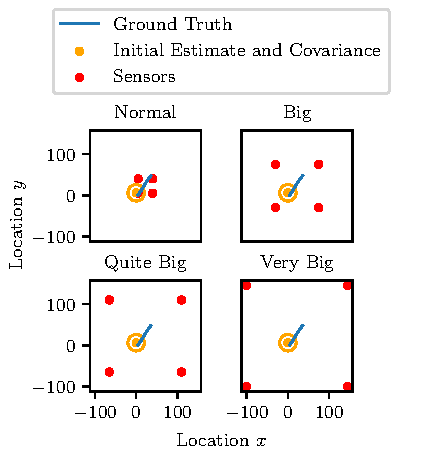
\includegraphics{figures/layouts.pdf}
    \caption{Different simulation layouts with varying distances between navigator and sensors.}
    \label{fig:sim_layouts}
\end{figure}
To demonstrate the accuracy of the method, we have compared the root mean square error (RMSE) of the privacy-preserving filter to the standard EIF using unmodified measurements, which is algebraically equivalent to the EKF typically used in industry for linearising non-linear state estimation. Estimation in each layout from figure \ref{fig:sim_layouts} consisted of $50$ filter iterations and was run $1000$ times. Unmodified measurement variances were taken as $r_{k,i}=5$ for all $k>0$ and a large fractional precision factor, $\phi=2^{32}$, was chosen. The results can be seen in figure \ref{fig:sim_layout_errors}.
\begin{figure}[htbp]
    \centering
    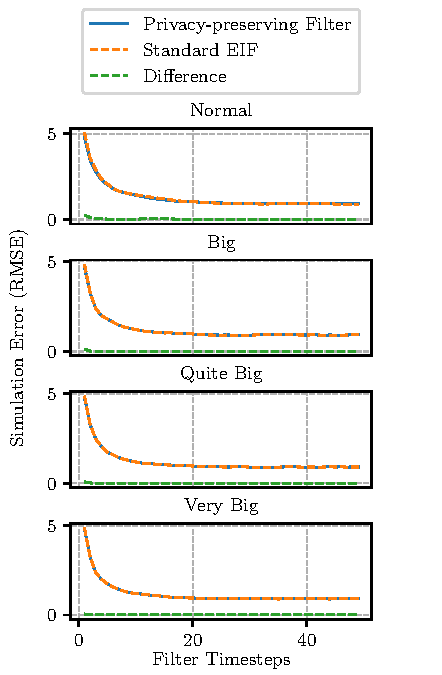
\includegraphics{figures/layout_errors.pdf}
    \caption{Average RMSE of our privacy-preserving filter and the standard EIF for different layouts.}
    \vspace{-\baselineskip}
    \label{fig:sim_layout_errors}
\end{figure}
From these results, we can see a strong similarity in filter performance between the privacy-preserving method and that of the traditional EIF. We can also see that the varying average distances between sensors and the navigator have little impact on the differences in performance. We attribute this similarity in RMSE to the conservativeness of estimated modified measurement variances $r'_{k,i}$, eliminating additional filter divergences, and to the high fractional precision factor, keeping computations consistent with the floating-point arithmetic of the EIF.

In addition to filter error, computational performance is important to consider when relying on cryptographic methods. Figure \ref{fig:sim_timing} shows the averages of $10$ execution times when varying the numbers of sensors and key sizes (bit lengths of $N$). Here, increasing the number of sensors primarily affects the number of inter-process communications and aggregation steps due to the asynchronous implementation.
\begin{figure}[htbp]
    \centering
    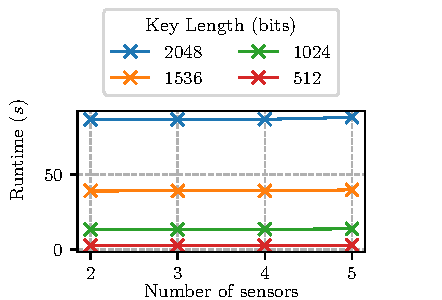
\includegraphics{figures/timing.pdf}
    \caption{Runtimes for varying key sizes and numbers of sensors.}
    \label{fig:sim_timing}
\end{figure}
We can see that the predominant computational costs stem from cryptographic computations and are directly dependent on the chosen key size. In practice, choosing a key size should take into account the duration of secrecy and the secret key lifetime. When relying on the DCRA for security, the current recommendation for encrypting government documents is the use of $2048$ bit length keys [barkerRecommendationPairwiseKey2019]. For our implementation and aforementioned hardware, this results in a filter update roughly every $1.7s$. In a scenario where sensors are mobile and past navigations can be made public, reduced key sizes can be considered, while a further decrease in computation time could be achieved with code optimisations and more powerful hardware.

% 
%  .d8888b.   .d88888b.  888b    888  .d8888b.  
% d88P  Y88b d88P" "Y88b 8888b   888 d88P  Y88b 
% 888    888 888     888 88888b  888 888    888 
% 888        888     888 888Y88b 888 888        
% 888        888     888 888 Y88b888 888        
% 888    888 888     888 888  Y88888 888    888 
% Y88b  d88P Y88b. .d88P 888   Y8888 Y88b  d88P 
%  "Y8888P"   "Y88888P"  888    Y888  "Y8888P"  
%                                               
%                                               
%                                               
% 

\section{Conclusions on Confidential Distributed Non-Linear Measurement Fusion}
We have presented a localisation filter in the presence of range-only sensors, which preserves both navigator and sensor privacies. A suitable cryptographic scheme has been introduced and a filter implementation compared and evaluated. Privacy-preserving range-only localisation is suitable for use in environments where sensor networks are untrusted or location is considered private and we hope to extend the method to broader measurement models in the future. Additional future work includes exploring more computationally efficient encryption schemes, the security implications of sensors that are not only honest-but-curious and expanding the LCAO notion to enforce the consistent broadcast assumption.